\documentclass[11pt,a4paper]{article}
\usepackage[margin=24mm]{geometry}
\usepackage{amsmath,amssymb,booktabs,array,graphicx}
\usepackage[T1]{fontenc}
\usepackage{lmodern}
\usepackage[hidelinks]{hyperref}
\hypersetup{pdftitle={Dilemma Dynamics: cooperation, deliberation and repeated-game incentives},pdfauthor={Alisa Sheinkman}}
\setlength{\parindent}{0pt}
\setlength{\parskip}{6pt}
\setlength{\emergencystretch}{3em}
\raggedbottom
\newcommand{\C}{\mathrm C}
\newcommand{\D}{\mathrm D}
\newcommand{\E}{\mathbb E}
\newcommand{\Prb}{\mathbb P}
\title{Dilemma Dynamics\\\large Cooperation, deliberation and repeated-game incentives}
\author{Alisa Sheinkman}
\date{Final evaluation and mathematical notes, 25 October 2026}
\begin{document}
\maketitle
\begin{abstract}
Cooperation can reward patience, but it can also be a costly mistake. Does an AI
that drafts before acting better recognise which situation it faces? Dilemma
Dynamics studies this question in repeated Prisoner's Dilemma games, where the
immediate gain from defection competes with the future value of reciprocity.
We compare immediate action with a bounded private draft in NVIDIA's Nemotron
Nano and Super at two sampling temperatures. Against disclosed opponent policies,
exact dynamic programming measures the payoff given up at each choice.
Autonomous pairings reveal how cooperation begins, breaks down and returns.
Matched game schedules, interleaved temperatures and durable event logs connect
aggregate comparisons to individual decisions. Drafting lowers average benchmark
loss for both models at both temperatures, yet increases loss against Tit-for-Tat.
Autonomous self-play also becomes less cooperative with drafting. The contrast
suggests that recognising immediate exploitation opportunities and sustaining
reciprocity are distinct capabilities. Temperature and action-label sensitivity
further qualify when deliberation helps. These notes connect the completed
results to repeated-game theory and propose targeted explanations for future tests.
\end{abstract}

\section{The question and the intervention}
The experiment asks whether a short deliberation procedure helps a model respond
to an opponent's incentives. Its two hosted models are Nemotron Nano and Super
\cite{nano,super}. The exact provider IDs, under the \texttt{nvidia/} namespace, are
\texttt{NVIDIA-Nemotron-3-Nano-30B-A3B} and
\texttt{nemotron-3-super-120b-a12b}.

\emph{Direct} makes one thinking-off action request, capped at 128 completion
tokens. \emph{Draft} makes a thinking-on request capped at 1,024 tokens, then a
separate thinking-off action request capped at 128 tokens \cite{cards}.
Both receive completed game history. Only the current decision's draft is added
to its action request. Each episode is assigned a sampling temperature
\(\tau\in\{0,1\}\); all its request phases use that value. The nucleus-sampling
setting is fixed at top-\(p=1\).
Each model--procedure combination is an experimental \emph{arm}.

Players maximise expected own cumulative points. Choices remain sealed until
joint reveal. Neutral X/Y labels use both mappings and display seats. In canonical
action labels, C means cooperate and D means defect:
\begin{center}
\begin{tabular}{lcc}
\toprule
Own action & Other cooperates & Other defects\\
\midrule
Cooperate & $(3,3)$ & $(0,5)$\\
Defect & $(5,0)$ & $(1,1)$\\
\bottomrule
\end{tabular}
\end{center}
Each pair lists (own points, other points). Write \(R=3\) for the mutual-cooperation
reward, \(S=0\) for cooperating against defection, \(T=5\) for defecting against
cooperation and \(P=1\) for mutual defection. These satisfy \(T>R>P>S\).

\clearpage
\section{Related literature and theoretical foundations}
Rasmusen's \emph{Games and Information} \cite{rasmusen} supplies the organising
ideas: strategies specify responses to histories, best responses maximise payoff
against a given opponent, and equilibrium requires compatible best responses.
Its treatment of finite and infinite repetition explains how the prospect of
another encounter changes present incentives. Its discussions of incomplete
information and the Axelrod tournament also motivate studying simple commitments
alongside adaptive players. Here those ideas lead to two complementary tracks:
exact payoff comparisons against disclosed policies, and observed interaction
between models whose policies emerge during play.

Akata et al.\ \cite{akata} study finitely repeated games with language models,
programmed strategies and human players. Their social chain-of-thought procedure
encourages a model to anticipate the other player's behaviour and improves
coordination in their experiments. This provides a close precedent for comparing
decision procedures. Dilemma Dynamics uses a bounded draft with a separate final
action request, making the procedure's token limits and request sequence explicit.

Fontana, Pierri and Aiello \cite{fontana} examine Llama2, Llama3 and GPT3.5 in
100-round Prisoner's Dilemma interactions against random opponents with different
cooperation probabilities. They check understanding of the rules and history and
find substantial variation in responses to opponent hostility. Their work
motivates our engineering checks and opponent-specific reporting. The present
benchmark adds an exact own-payoff reference for each disclosed commitment,
allowing cooperation and decision quality to be examined separately.

Pal et al.\ \cite{pal} infer strategies from decisions across possible recent
histories, vary continuation probabilities, payoffs, horizons and framing, and
assess equilibrium properties. Their approach emphasises the value of observing
responses to histories that ordinary play may rarely visit. Our autonomous track
records realised trajectories; its cooperation, breakdown and recovery statistics
describe the interaction paths actually sampled.

Taylor and Bergen \cite{taylor} study action--message incongruence in games with
a communication phase. They vary the incentives and timing of messages and
report associations between reasoning performance and misrepresentation.
This places the present intervention in a wider behavioural context: payoff
competence, cooperation and truthful communication are distinct properties of
an agent. Our sealed-action design concentrates on the first two.

Together, these studies motivate a question about \emph{when} deliberation helps:
a change in average score may combine better exploitation of an unresponsive
opponent, better preservation of reciprocity and different behaviour under
uncertainty. The disclosed-policy track exposes those components, while matched
temperature comparisons test their sensitivity to the sampling setting.

\clearpage
\section{Repetition and the value of a future encounter}
An \emph{episode} is one complete interaction between two players. Round number
is \(t=1,2,\ldots\), and \(N\) denotes the total number of rounds in that episode.
In a fixed-horizon episode, \(N=H\), where the positive integer \(H\) is announced
before play. In a geometric episode, continuation probability \(\delta\) satisfies
\(0\leq\delta<1\). After each completed round, the game continues with probability
\(\delta\) and ends with probability \(1-\delta\), independently of the actions.

One equivalent construction draws an independent uniform variable
\(U_t\sim\operatorname{Uniform}(0,1)\) after round \(t\), continuing precisely when
\[
U_t<\delta.
\]
The realised length then has distribution and mean
\begin{equation}
\Prb(N=n)=(1-\delta)\delta^{n-1},\qquad
\Prb(N\geq t)=\delta^{t-1},\qquad
\E[N]=\frac{1}{1-\delta},\quad n,t\geq1.
\label{eq:stopping}
\end{equation}
For \(\delta=0\), the game lasts one round. The first survival probability is one.
Thus \(\delta=.9\) produces ten expected rounds, with a hidden last round; an
announced ten-round horizon gives players different information. The executable
scheduler uses seeded, exact rational draws for the specified probabilities.
Matched treatments reuse the same environment draws.

\subsection{Committed responses}
The disclosed opponents are AllC (always C), AllD (always D), Tit-for-Tat (C first,
then the subject's preceding action) and Grim (C until a subject defection,
then D forever). This makes the consequences of a current action computable.
Rasmusen's distinction between a commitment and strategic equilibrium is useful
here \cite[Sections 4.1 and 5.1--5.2]{rasmusen}.

Against untriggered Grim, cooperation forever has value \(R/(1-\delta)\).
Defecting now, followed by the best response to permanent punishment, has value
\(T+\delta P/(1-\delta)\). Cooperation is weakly preferable exactly when
\begin{equation}
\frac{R}{1-\delta}\geq T+\frac{\delta P}{1-\delta}
\quad\Longleftrightarrow\quad
\delta\geq\frac{T-R}{T-P}=\frac12.
\label{eq:grim}
\end{equation}
All four payoff symbols were defined with the matrix; \(\delta\) is the chance
of another round. Equality allows both initial choices to be optimal.

Against initially cooperating Tit-for-Tat, three continuation patterns determine
the optimal initial value: cooperate forever, defect forever, or alternate D,C.
Their respective values are
\[
\frac{3}{1-\delta},\qquad 5+\frac{\delta}{1-\delta},\qquad
\frac{5}{1-\delta^2}.
\]
The alternating pattern earns 5,0 repeatedly. Comparing all three shows that
initial cooperation is optimal for \(\delta\geq2/3\). The tested probabilities
.4, .6 and .9 therefore span different incentive regimes.

\clearpage
\section{Exact payoff references and decision loss}
Track A tests each disclosed policy at all three continuation probabilities.
One-round AllC/AllD and announced ten-round Tit-for-Tat/Grim complete 16 conditions.
For any condition, let \(s\) be the opponent's relevant memory state,
\(a\in\{\C,\D\}\) the subject's action, \(r(s,a)\) the resulting own payoff and
\(f(s,a)\) the next opponent state. Let \(V^*(s)\) be the maximum achievable
expected total own payoff from state \(s\); \(Q^*(s,a)\) fixes the current action
and allows optimal choices thereafter. In a geometric episode,
\begin{equation}
Q^*(s,a)=r(s,a)+\delta V^*(f(s,a)),\qquad
V^*(s)=\max_{a\in\{\C,\D\}}Q^*(s,a).
\label{eq:bellman}
\end{equation}
The implementation uses rational arithmetic. It certifies a candidate value
function by checking \(V^*(s)\geq r(s,a)+\delta V^*(f(s,a))\) for every state and
action, with equality for at least one action in each state.

For a finite game, let \(h\) be rounds remaining, including the current one.
Backward induction starts at \(V^*_0(s)=0\) and applies
\[
Q^*_h(s,a)=r(s,a)+V^*_{h-1}(f(s,a)),\qquad
V^*_h(s)=\max_a Q^*_h(s,a).
\]
Against committed ten-round Tit-for-Tat or Grim, the optimal initial path is nine
C moves followed by D, earning \(9R+T=32\) points. The standard finite-game
backward-induction argument in which both players remain free to optimise uses
a different opponent model \cite[Section 5.1]{rasmusen}.

At a revealed decision, \(s_t\) is the pre-action opponent state and \(a_t\) the
chosen action. Its nonnegative payoff gap is
\[
g_t=V^*(s_t)-Q^*(s_t,a_t),
\]
with the corresponding remaining-horizon values in a finite episode. Episode
losses are
\begin{equation}
L_{\rm geometric}=(1-\delta)\sum_{t=1}^{N}g_t,\qquad
L_{\rm fixed}=\frac{1}{H}\sum_{t=1}^{H}g_t.
\label{eq:loss}
\end{equation}
Zero gap means that the current action preserves optimal achievable payoff.
For example, C against AllC in a one-round game gives up \(T-R=2\) points;
D has gap zero. Loss is expressed in normalised own-payoff points.

Equation~\eqref{eq:stopping} explains the geometric weighting: survival to round
\(t\) already occurs with probability \(\delta^{t-1}\). The expectation of the
realised sum in \eqref{eq:loss} therefore includes that survival factor. Applying
it again to each recorded gap would count stopping twice.

Track B tests all ten unordered pairings of the four arms, including self-play,
at \(\delta=.9\). Here outcomes of interest are cooperation and joint return.
For player \(i\in\{1,2\}\), write \(r_{i,t}\) for points in round \(t\). A dyad's
normalised joint return is \((1-\delta)\sum_{t=1}^{N}(r_{1,t}+r_{2,t})\).
We report first-round mutual cooperation, cooperation per observed round and
per episode, and breakdown/recovery counts with opportunity denominators.
Long episodes receive more weight in a pooled round rate; rounds in one dyad
share a history and are statistically dependent.

\clearpage
\section{Replication and statistical comparisons}
A block groups the related experimental conditions and arms. Each block has
64 Track A episodes (16 conditions for each of four arms) and ten Track B dyads
per temperature. The frozen resource-only selection chose 48 blocks at each
temperature: 6,144 benchmark episodes and 960 autonomous dyads, or 7,104 episodes
in total. Four strata, defined by action-label mapping and display seat, each
contain 12 blocks per temperature.

A fresh master seed fixes game schedules and order. Arms within a block share
environment draws, and corresponding temperature episodes are adjacent in a
frozen randomised order. This pairing controls stopping and presentation
variation while spreading both temperatures through the same service window.
Nested 24/32/48-block candidates were frozen before engineering; measured token
use and latency selected the largest fitting candidate before scientific
inference. Selection uses resource telemetry alone.

\subsection{Primary drafting effects}
Write \(L_{m,k,\tau,b,c}\) for Track A loss in model \(m\in\{\mathrm{Nano},\mathrm{Super}\}\),
procedure \(k\in\{\mathrm{Direct},\mathrm{Draft}\}\), temperature \(\tau\in\{0,1\}\),
block \(b\) and condition \(c\in\{1,\ldots,16\}\). The block's condition mean is
\[
\bar L_{m,k,\tau,b}=\frac1{16}\sum_{c=1}^{16}L_{m,k,\tau,b,c}.
\]
For the contrast under consideration, let \(\mathcal B_j\) be the set of blocks
in stratum \(j\in\{1,2,3,4\}\) with complete observations for both procedures;
\(|\mathcal B_j|\) denotes its size. The drafting effect is
\begin{equation}
\Delta_{m,\tau}=\frac14\sum_{j=1}^{4}\frac1{|\mathcal B_j|}
\sum_{b\in\mathcal B_j}\left(\bar L_{m,\mathrm{Draft},\tau,b}
-\bar L_{m,\mathrm{Direct},\tau,b}\right).
\label{eq:primary}
\end{equation}
Negative values favour Draft. All conditions and strata have equal weight.
The completed design has \(|\mathcal B_j|=12\) in every stratum.
The point estimate requires at least one complete paired block in every stratum.

There are four primary contrasts, one for each model and temperature. Use
50,000 deterministic PCG64 bootstrap replicates, resampling whole blocks within
strata. For family error level \(\alpha=.05\) and \(K=4\) contrasts, each marginal
interval has nominal coverage \(1-\alpha/K=.9875\). Its bootstrap quantiles are
\(\alpha/(2K)=.00625\) and \(1-\alpha/(2K)=.99375\). This Bonferroni allocation
uses approximate bootstrap coverage. At least five complete paired blocks per
stratum are required to construct an interval.

\subsection{Temperature comparisons and missingness}
Six secondary contrasts compare temperature 0 minus 1 for each of the four arms,
and \(\Delta_{m,0}-\Delta_{m,1}\) for each model. A positive value of the latter
means a smaller drafting advantage at zero. Resampling uses the same matched
block indices jointly across temperatures; secondary 95\% intervals are nominal.

Every scheduled episode retains a status. Estimates from complete blocks are
conditional on their completion. Dynamic programming bounds feasible loss over
the remaining scheduled rounds, given any committed prefix. These bounds describe
the finite schedule's missingness exposure. The release gate requires completion
of both temperatures before the public report and app change over.

\clearpage
\section{Evidence, execution and interpretation}
The local CPU coordinates remote Nebius Token Factory inference. Inspect AI
provides native samples, model events and custom scored outcomes \cite{inspect}.
The audited gateway owns HTTP transmission, reservations and recovery; native
joint-reveal events carry hashes linking them to the canonical event chain.
MLflow Skinny records run identities, parameters, metrics and artifacts in local
SQLite \cite{mlflow}. NumPy supplies the bootstrap, PyArrow numeric Parquet
exports and Matplotlib the primary comparison figure.

The evidence packet retains append-only requests and revealed rounds, native
Inspect logs, accounting, statuses and exports. Offline reconstruction produces
episode histories, decision/request tables, condition means, contrasts and
checksums. The dependency lock and runtime manifest record the installed state;
source archives preserve the executed implementation. Private responses and
drafts remain local.

\subsection{Bounded recovery}
The additional campaign ceiling is \$40: \$2 engineering, \$34 final inference,
\$2 other-charge reserve and \$2 contingency. Retry exposure is included in stage
allocations. Reservations precede transmission, and ambiguous requests retain
their exposure. Durable valid responses are replayed. A successful but invalid
response stays in the record and ends its admitted scientific observation.

A provider-overload interruption led to an explicitly approved transport
amendment: six total attempts per logical request, one durable 30-minute recovery
window per decision, a shared five-minute overload cooldown, and two sample
workers sharing four request slots. The original campaign deadline remains
36 hours, with its watchdog and shutdown margin. The original source and ledger
prefix remain intact; a separate frozen receipt records the amendment.

\subsection{Completion, accounting and reproducibility}
All 7,104 scientific episodes completed, with 3,552 at each temperature.
The scientific stage ran from 24 October 2026, 14:10 UTC, to 25 October,
06:20 UTC (16.16 elapsed hours, including the interruption).
The recovery preserved all 3,406 previously completed episodes and the original
ledger prefix. There were 62,832 successful requests and 20 additional transmitted
attempts: 17 HTTP 529 responses, one HTTP 502 and two attempts without a durable
HTTP response. No scheduled observation is missing.

Usage-priced final inference is estimated at \$17.15200728 and engineering at
\$0.63490812. Another \$0.32479584 remains reserved against the 20 uncertain
transmissions. Thus campaign inference exposure is at most \$18.11171124 under
these recorded bounds, before the \$4 non-inference/contingency allocation.
These figures are not provider invoices. On 25 October the user explicitly
approved publication with this unresolved maximum exposure disclosed. The
original accounting gate still reports unresolved reservations; the separate
publication amendment changes only that release condition. No reservation or
usage record was cleared or relabelled.

Native Inspect scored-sample coverage, canonical reconstruction, frozen original
and recovery source, and final MLflow evidence heads were verified. Public actions
reproduce exact scores and bootstrap comparisons offline. Numerical request and
decision tables support the usage diagnostics; private draft text and raw native
logs remain in the evidence archive. Hosted replay is not required to reproduce
the released statistics. Public hashes provide integrity checks rather than
independent authentication of private provider evidence.

\clearpage
\section{Results: better decisions against whom?}
Each model--procedure arm has 768 benchmark episodes at each temperature.
Table~\ref{tab:primary} gives the four planned primary comparisons; lower loss
means less achievable expected own payoff forgone. The intervals use the
pre-specified approximate four-comparison family treatment described above.
Every interval lies below zero. Relative to each Direct mean, the reductions
are 16.8\%, 19.4\%, 25.7\% and 37.5\%, respectively. These percentages describe
loss reduction, not a percentage increase in earned reward.

\begin{table}[htbp]\centering\small
\begin{tabular}{lrrrrl}
\toprule
Model & $\tau$ & Direct & Draft & Draft--Direct & 98.75\% interval\\
\midrule
Nano & 0 & .6462 & .5374 & $-.1088$ & [$-.1640,-.0577$]\\
Super & 0 & .4616 & .3720 & $-.0896$ & [$-.1212,-.0591$]\\
Nano & 1 & .6541 & .4861 & $-.1680$ & [$-.2172,-.1209$]\\
Super & 1 & .5988 & .3741 & $-.2246$ & [$-.2795,-.1742$]\\
\bottomrule
\end{tabular}
\caption{Planned benchmark comparisons in normalised payoff points. All 48
matched blocks contribute, with 12 blocks in each presentation stratum.}
\label{tab:primary}
\end{table}

\begin{center}
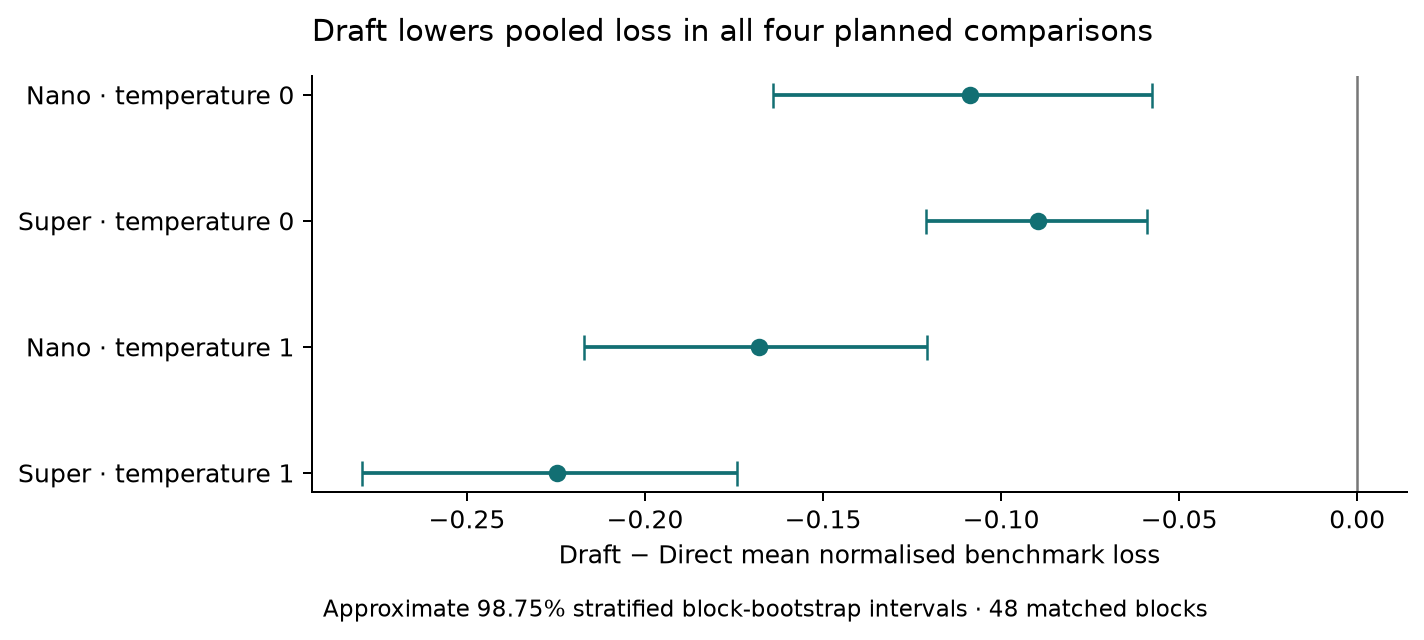
\includegraphics[width=.98\linewidth]{../figures/primary-results.png}
\end{center}

\subsection{The average hides a Tit-for-Tat reversal}
Against Always Cooperate, drafting reduces loss by .5865 and .6042 for Nano
at temperatures zero and one, and by .2094 and .5167 for Super. Against this
unresponsive opponent, D is optimal at every round: an improvement therefore
means more effective exploitation, rather than more cooperation. Super Draft
also nearly eliminates loss against Always Defect. Nano Draft at temperature
zero has a small opposite aggregate change against Always Defect ($+.0068$).

Against Tit-for-Tat the sign reverses for every model and temperature
(Table~\ref{tab:policy}). The reversal is concentrated in continuation .6, .9
and the announced ten-round game; at .4 drafting improves all four means.
The .6 case rewards alternation, whereas .9 rewards sustained cooperation.
Worse loss in both regimes indicates that a uniform instruction to cooperate
more, or to defect more, would not explain all the errors. The 16-condition
breakdown in Figure~\ref{fig:conditions} prevents gains against simple policies
from concealing these difficulties.

\begin{table}[htbp]\centering\small
\begin{tabular}{lrrrr}
\toprule
Opponent & Nano 0 & Super 0 & Nano 1 & Super 1\\
\midrule
Always Cooperate & $-.5865$ & $-.2094$ & $-.6042$ & $-.5167$\\
Always Defect & $+.0068$ & $-.2083$ & $-.1984$ & $-.3385$\\
Grim & $-.0958$ & $-.1511$ & $-.1919$ & $-.2151$\\
Tit-for-Tat & $+.2404$ & $+.2103$ & $+.3225$ & $+.1717$\\
\bottomrule
\end{tabular}
\caption{Exploratory Draft--Direct mean losses by opponent, averaging its four
conditions equally (192 episodes per arm/opponent/temperature).}
\label{tab:policy}
\end{table}

\begin{figure}[p]\centering
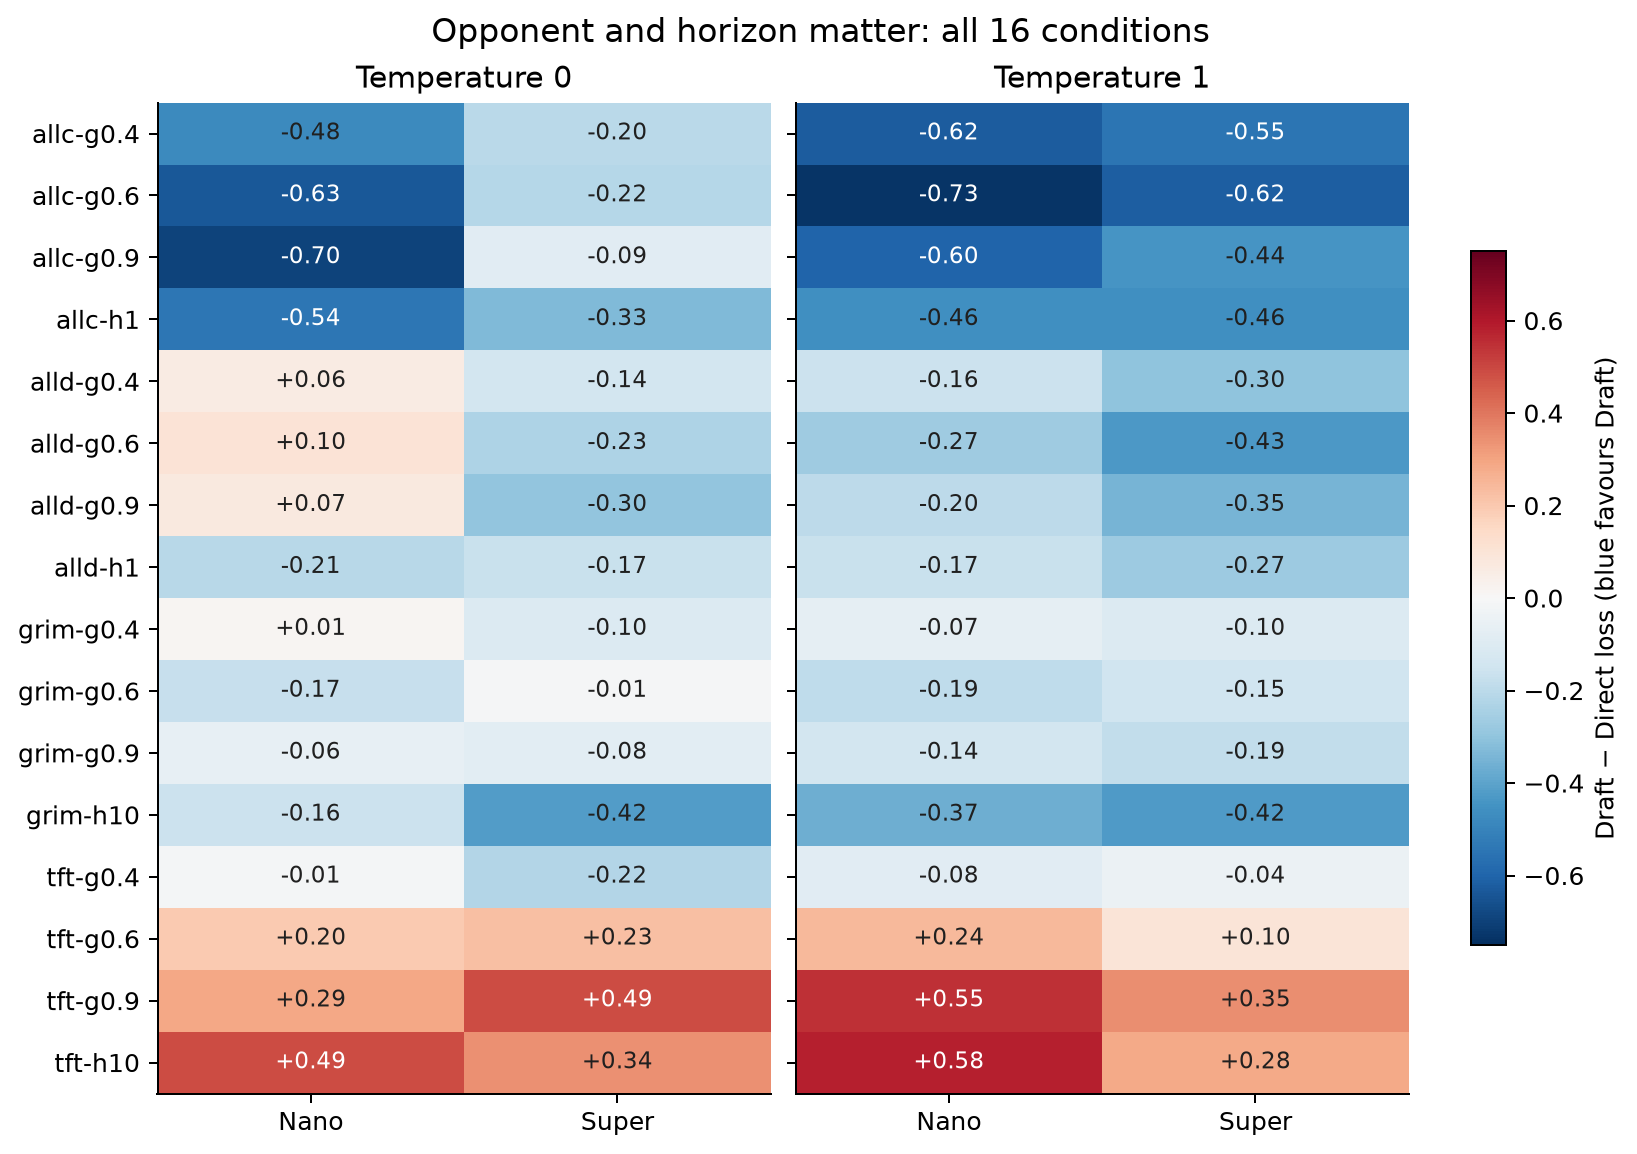
\includegraphics[width=\linewidth]{../figures/condition-effects.png}
\caption{All condition effects, chosen for disclosure rather than significance.
Blue favours Draft; red favours Direct. Each cell compares 48 episodes per arm.
Condition codes g denote geometric continuation; h denotes announced length.
These exploratory point estimates have no simultaneous uncertainty guarantee.}
\label{fig:conditions}
\end{figure}

\subsection{Temperature changes the drafting advantage}
The six planned secondary contrasts use nominal approximate 95\% intervals.
For Super Direct, temperature zero minus one is $-.1372$
[$-.1814,-.0942$], while Super Draft changes by $-.0022$
[$-.0193,+.0147$]. Nano Direct changes by $-.0080$
[$-.0480,+.0316$], and Nano Draft by $+.0513$ [$+.0199,+.0815$].
Thus zero temperature improves one Direct procedure markedly, worsens one Draft
procedure, and leaves two contrasts near zero relative to their uncertainty.
The Draft--Direct advantage narrows at zero for Nano by $+.0592$
[$+.0099,+.1084$] and for Super by $+.1350$ [$+.0876,+.1849$].
These six intervals were not multiplicity adjusted. Temperature has no uniform
preferred setting across the four arms.

\subsection{Presentation sensitivity and finite planning}
An exploratory presentation slice reveals a large Nano effect at temperature
zero. When X means C, Draft--Direct loss is $-.4652$ in the first display seat
and $-.2558$ in the second; when X means D, it is $+.1427$ and $+.1431$.
Each stratum has 12 blocks. Seats show the same mapping-associated reversal,
while Nano's temperature-one effects and all Super effects favour Draft in
every stratum. Strata also have different stopping draws, so these estimates
motivate a fully crossed label experiment rather than isolating a causal label
effect. Equal weighting of all four strata is essential to the reported average.

In the ten-round committed-policy games, the optimal own action path is nine C
moves followed by D, with total payoff 32. Across all 768 such episodes,
only one follows that path (Super Draft against Grim at temperature zero).
Against TFT, Super Draft cooperates in round nine in 43/48 temperature-zero
episodes and defects in round ten in all 48, yet never follows the complete
optimal path. Its actions match a useful local endgame in many histories while
losing payoff earlier. Against Grim at continuation .9, even Super Draft starts
with the optimal C in only 26/48 episodes at zero and 17/48 at one. This is a substantial gap in sustained contingent planning despite improvement
on the pooled benchmark.

\clearpage
\section{Autonomous interaction: cooperation is a separate outcome}
Every unordered pairing has 48 dyads and 376 realised rounds per temperature.
Across all ten pairings, mutual cooperation occurs in 330/3,760 rounds (8.8\%)
at zero and 353/3,760 (9.4\%) at one. The corresponding means of within-episode
CC fractions are 8.9\% and 9.8\%. These two weighting schemes answer different
questions; rounds in a trajectory are dependent.

\begin{table}[htbp]\centering\small
\begin{tabular}{lrrrr}
\toprule
Self-play arm & CC rounds, $\tau=0$ & $J$, $\tau=0$ & CC rounds, $\tau=1$ & $J$, $\tau=1$\\
\midrule
Nano Direct & 61/376 & 2.7500 & 87/376 & 3.3729\\
Nano Draft & 29/376 & 2.5083 & 15/376 & 2.3854\\
Super Direct & 124/376 & 3.2063 & 58/376 & 3.1500\\
Super Draft & 3/376 & 1.8667 & 9/376 & 2.0792\\
\bottomrule
\end{tabular}
\caption{Self-play cooperation and mean normalised joint return $J$.
Draft lowers both point estimates for each model at each temperature.}
\label{tab:self}
\end{table}

\begin{center}
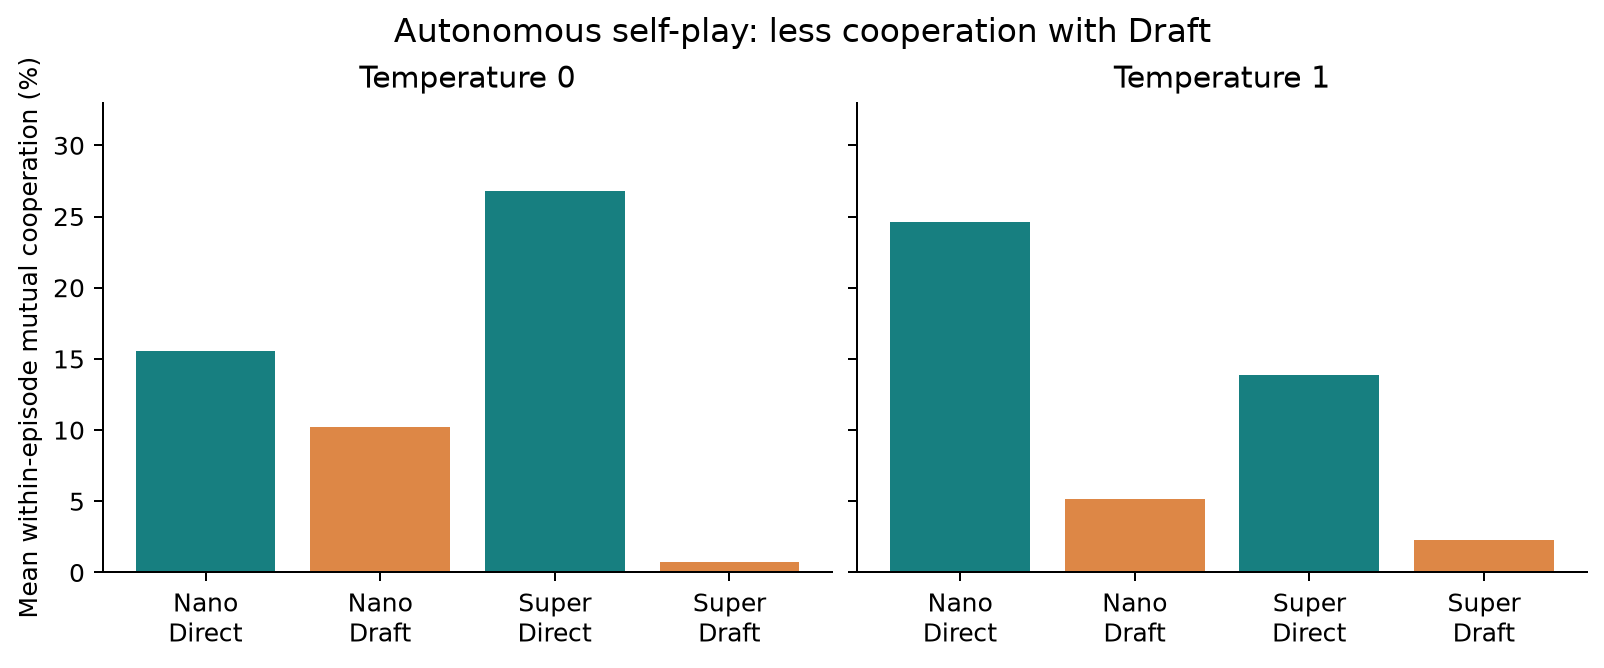
\includegraphics[width=\linewidth]{../figures/autonomous-self-play.png}
\end{center}

For Super at zero, changing both self-play agents from Direct to Draft lowers
mean normalised joint return by 1.3396 (exploratory nominal 95\% paired-block
interval [$-1.8375,-.9042$]). Super Draft self-play has 329/376 DD rounds,
three first-round CC outcomes, and no return to CC in 325 opportunities.
Super Direct self-play starts with zero first-round CC outcomes but later
recovers CC in 82/218 eligible transitions. Its 124 CC rounds show that low
initial cooperation can coexist with subsequent coordination.

The other self-play joint-return differences (Draft minus Direct) are
$-.2417$ [$-.5458,+.0271$] for Nano at zero,
$-.9875$ [$-1.3063,-.6958$] for Nano at one, and
$-1.0708$ [$-1.4208,-.7521$] for Super at one.
These post-viewing comparisons change both players together and have no
multiplicity correction. All ten pairings, including cross-model interactions,
are released with CC/CD/DC/DD counts and breakdown/recovery opportunities.

The shared realised .9-continuation schedule averages 7.833 rounds, below its
population expectation of ten. On this particular schedule, constant CC would
yield mean $J=4.7000$, and constant DD $J=1.5667$. This helps interpret the
normalised returns without mistaking a realised average for a population limit.

\section{Compute, transport and explanatory hypotheses}
\subsection{The intervention has a material resource cost}
At each temperature every arm contributes 5,236 decisions across both tracks.
Direct needs one successful request per decision and Draft two. Within a model,
Draft's recorded final usage costs are about 10.0--11.9 times Direct's; these
costs include autonomous play as well as benchmark episodes.
Median request latency ranges from .36--.69 seconds for Direct and .96--1.98
seconds for the mixture of Draft's two request phases. Summing phase latencies,
queueing and cooldowns is necessary to estimate decision or wall-clock delay;
the mixed per-request median is not that quantity.

The thinking draft hits its 1,024-token cap in 1,322/5,236 Nano-zero drafts
(25.2\%), 2,148/5,236 Nano-one (41.0\%), 1,941/5,236 Super-zero (37.1\%)
and 2,938/5,236 Super-one (56.1\%). Completion tokens include the provider's
counted output; missing reasoning-token detail is not evidence of zero reasoning.
This study therefore evaluates a frequently truncated bounded procedure.
Cap status is an outcome of the request and its difficulty, so a capped versus
uncapped comparison would be confounded.

Successful responses report the requested model identifier and one fingerprint
per model. These identifiers do not pin weights or hidden serving state. Listed
regions, quantisations and prices differ between models, so absolute model
differences also combine serving differences.

The transport amendment changes concurrency and waiting. Original/recovery loss
means are disclosed, but segment composition differs and two episodes span the
interruption. These slices cannot isolate recovery effects or backend drift.

\subsection{Hypotheses suggested by the observations}
\begin{enumerate}
\item \textbf{Local optimisation outruns contingent planning.} Near-zero Super
Draft loss against unresponsive policies, TFT reversals and rare optimal
finite paths suggest that simple exploitation is easier than preserving future
responses. A future test could hold token budget fixed and vary the depth of
explicit state-transition planning, scoring first actions and continuation
choices separately.
\item \textbf{Independent defensive choices create a low-cooperation trap.}
Super Draft's low self-play CC and zero observed CC recovery at temperature zero
suggest a mechanism in which individually cautious play blocks reciprocal
exploration. A controlled partner policy that forgives after a fixed number of
D rounds could test whether repair opportunities restore cooperation. The
present action-only protocol does not identify latent fear or intent.
\item \textbf{Deliberation can partly stabilise or amplify presentation habits.}
Nano-zero's mapping-associated sign reversal and weaker temperature-one
sensitivity motivate crossing every seed with every mapping and seat. This
would separate presentation from the current stratum-specific stopping draws.
\item \textbf{Truncation and temperature interact with the two-stage procedure.}
More cap hits at temperature one coexist with better Nano Draft loss but almost
unchanged Super Draft loss. A future cap randomisation and equal-compute Direct
control would distinguish output budget from sampling and draft conditioning.
\end{enumerate}

Bounded drafting improves mean exact payoff decisions over this balanced
benchmark while leaving reciprocity and planning failures visible in autonomous
play. The hypotheses above suggest future tests; no further paid calls are
required to reproduce this final evaluation.

\clearpage
\appendix
\section{Probabilities and the app's forecast inequality}
The optional app protocol asks for an opponent-action forecast and two conditional
future-payoff forecasts. These are elicited separately from the final evaluation's
action-only scientific requests. Their algebra helps explain the difference
between immediate temptation and future incentives.

Let \(\mathcal H_t\) be the completed history available before round \(t\), and
let \(p_t\in[0,1]\) be the reported probability that the opponent cooperates in
that round. Thus \(p_t\) concerns the opponent's \emph{current action}; \(\delta\)
concerns whether a \emph{later round exists}. The simultaneous protocol keeps
the opponent's current choice sealed while the subject chooses.

Let \(F_{a,t}\) be the reported expected own total from the next round onward,
conditional on continuation and on choosing \(a\in\{\C,\D\}\) now. It includes
future opponent responses and subsequent stopping. Whenever no further round
is possible, define \(F_{a,t}=0\). The probability of reaching the next round is
\[
\rho_t=\begin{cases}
\delta, & \text{geometric game},\\
1, & \text{fixed game with }t<H,\\
0, & \text{fixed game with }t=H.
\end{cases}
\]
The conditional future totals have bounds
\[
0\leq F_{a,t}\leq
\begin{cases}
5/(1-\delta),&\text{geometric game},\\
5(H-t),&\text{fixed game},
\end{cases}
\]
because five is the maximum own payoff per round. In the geometric case,
conditioning on the next round means the remaining expected length is again
\(1/(1-\delta)\).

Write \(\widehat Q_t(a)\) for expected own payoff according to these submitted
forecasts. With the payoff matrix in Section~1,
\begin{align*}
\widehat Q_t(\C)&=p_tR+(1-p_t)S+\rho_tF_{\C,t}
=3p_t+\rho_tF_{\C,t},\\
\widehat Q_t(\D)&=p_tT+(1-p_t)P+\rho_tF_{\D,t}
=1+4p_t+\rho_tF_{\D,t}.
\end{align*}
Cooperation is weakly preferred according to the forecasts precisely when
\begin{equation}
\rho_t\bigl(F_{\C,t}-F_{\D,t}\bigr)\geq1+p_t.
\label{eq:forecast}
\end{equation}
The right side is the immediate gain from defection, between one and two points;
the left side is cooperation's forecast future advantage, weighted by the chance
of reaching that future. Equality means a tie. At an announced final round,
\(\rho_t=0\), so the immediate incentive favours D for every \(p_t\in[0,1]\).

This check measures consistency between an action and submitted forecasts.
Forecast accuracy can then be studied against outcomes that were actually
observed. A one-step counterfactual holds the other player's sealed current
action fixed; a longer alternative history requires specifying how that opponent
would respond.

\clearpage
\section{Competitive board-game calculations}
The app's visible sequential board games provide additional examples of tactics
and exact search. They use separate rules and analyses from the cooperation
study.

\subsection{Tic-tac-toe}
Let \(x\) denote a board state including the player to move, \(A(x)\) its legal
moves and \(f(x,a)\) the state after move \(a\). Let \(G(x)\) be optimal game value
from the current player's perspective. Terminal values are win \(+1\), draw 0
and loss \(-1\), according to that same perspective. Because each move passes
the turn, a nonterminal state satisfies
\[
G(x)=\max_{a\in A(x)}[-G(f(x,a))].
\]
The game is small enough for exhaustive minimax. Legality, search value and the
player's explanation can therefore be checked separately.

\subsection{Dots \& Boxes}
Here \(x\) includes drawn edges, box ownership and the player to move. Write
\(g(x,a)\) for the number of boxes captured by drawing edge \(a\), and \(W(x)\)
for optimal remaining-box difference from the current player's perspective.
An edge that captures a box grants another turn. Thus
\[
W(x)=\max_{a\in A(x)}\left[g(x,a)+\sigma(x,a)W(f(x,a))\right],\qquad
\sigma(x,a)=\begin{cases}+1,&g(x,a)>0,\\-1,&g(x,a)=0.\end{cases}
\]
At a terminal state, \(W(x)=0\), since no boxes remain. The difference in boxes
already owned is added separately to obtain the final score difference.
The positive sign preserves perspective after an extra turn; the negative sign
switches it when the turn passes.

Exact edge search is used within explicit state and computation limits, with
incomplete searches labelled unknown. Restricted long-chain/loop endgames also
admit specialised references. A box sacrifice can preserve control and increase
the eventual score; its value depends on the remaining position and the validity
of that reference's assumptions.

Both board games have competitive outcomes: a gain in the score difference is a
loss for the other player. The repeated dilemma adds the possibility that future
mutual cooperation improves both players' returns. This makes it useful to
present tactical foresight and cooperation incentives as separate examples.

\clearpage
\begin{thebibliography}{10}
\raggedright
\bibitem{rasmusen}
Eric Rasmusen. \emph{Games and Information: An Introduction to Game Theory}.
4th ed., Blackwell Publishing, 2007. Relevant discussions: Sections 1.2, 4.1,
5.1--5.2 and 6.4--6.5. Research preparation also used the supplied fourth-edition
draft with chapter headers dated 2005.
\href{https://rasmusen.org/GI/}{Author's book materials}.

\bibitem{akata}
Elif Akata, Lion Schulz, Julian Coda-Forno, Seong Joon Oh, Matthias Bethge and
Eric Schulz. \emph{Playing repeated games with large language models}.
\emph{Nature Human Behaviour}, 2025.
\href{https://doi.org/10.1038/s41562-025-02172-y}{doi:10.1038/s41562-025-02172-y}.
\href{https://arxiv.org/abs/2305.16867v2}{arXiv:2305.16867v2}, revised 7 May 2025.

\bibitem{fontana}
Nicol\`o Fontana, Francesco Pierri and Luca Maria Aiello.
\emph{Nicer Than Humans: How do Large Language Models Behave in the Prisoner's Dilemma?}
\href{https://arxiv.org/abs/2406.13605v2}{arXiv:2406.13605v2}, 19 September 2024.

\bibitem{pal}
Saptarshi Pal, Abhishek Mallela, Christian Hilbe, Lenz Pracher, Chiyu Wei,
Feng Fu, Santiago Schnell and Martin A. Nowak.
\emph{Strategies of cooperation and defection in five large language models}.
\href{https://arxiv.org/abs/2601.09849v1}{arXiv:2601.09849v1}, 14 January 2026.

\bibitem{taylor}
Samuel M. Taylor and Benjamin K. Bergen.
\emph{When Do Large Language Models Exhibit Unsolicited Deception?}
\emph{Transactions of the Association for Computational Linguistics},
14:1936--1962, 2026. \href{https://doi.org/10.1162/TACL.a.786}{doi:10.1162/TACL.a.786}.
\href{https://arxiv.org/abs/2504.00285v2}{arXiv:2504.00285v2}, revised 9 September 2026.

\bibitem{nano}
NVIDIA. \emph{Nemotron 3 Nano: Open, Efficient Mixture-of-Experts Hybrid
Mamba-Transformer Model for Agentic Reasoning}.
\href{https://research.nvidia.com/labs/nemotron/files/NVIDIA-Nemotron-3-Nano-Technical-Report.pdf}{Technical report}, 23 December 2025.

\bibitem{super}
NVIDIA. \emph{Nemotron 3 Super: Open, Efficient Mixture-of-Experts Hybrid
Mamba-Transformer Model for Agentic Reasoning}.
\href{https://research.nvidia.com/labs/nemotron/files/NVIDIA-Nemotron-3-Super-Technical-Report.pdf}{Technical report}, 3 April 2026 revision.

\bibitem{cards}
NVIDIA. \emph{Nemotron 3 model cards and inference documentation}:
\href{https://huggingface.co/nvidia/NVIDIA-Nemotron-3-Nano-30B-A3B-BF16}{Nano 30B-A3B-BF16};
\href{https://huggingface.co/nvidia/NVIDIA-Nemotron-3-Super-120B-A12B-BF16}{Super 120B-A12B-BF16}.
Thinking controls; accessed 24 October 2026.

\bibitem{inspect}
UK AI Security Institute. \emph{Inspect AI: Log Files}.
\url{https://inspect.aisi.org.uk/eval-logs.html}. Accessed 24 October 2026.

\bibitem{mlflow}
MLflow contributors. \emph{MLflow Tracking documentation}.
\url{https://mlflow.org/docs/latest/tracking/}. Accessed 24 October 2026.
\end{thebibliography}
\end{document}
